\documentclass[fleqn, a4paper, 11pt, oneside]{amsart}
%\usepackage[top = 2cm, bottom = 1cm, left = 1cm, right = 1cm]{geometry}
\usepackage{exsheets, tasks}
\usepackage{amsmath, amssymb, amsthm} %standard AMS packages
\usepackage{marginnote} %marginnotes
\usepackage{gensymb} %miscellaneous symbols
\usepackage{commath} %differential symbols
\usepackage{xcolor} %colours
\usepackage{cancel} %cancelling terms
\usepackage[free-standing-units, space-before-unit]{siunitx} %formatting units
	\sisetup
	{
		per-mode=fraction,
		fraction-function=\frac
	}
\usepackage{tikz, pgfplots} %diagrams
\usetikzlibrary{calc, hobby, patterns, intersections, decorations.markings}
\usepackage{graphicx} %inserting graphics
\usepackage{hyperref} %hyperlinks
\usepackage{datetime} %date and time
\usepackage{ulem} %underline for \emph{}
\usepackage{xfrac} %inline fractions
\usepackage{enumerate,enumitem} %numbered lists
\usepackage{float} %inserting floats
\usepackage{circuitikz}[american voltages, american currents] %circuit diagrams
\usepackage[utf8]{inputenc}

\newcommand\numberthis{\addtocounter{equation}{1}\tag{\theequation}} %adds numbers to specific equations in non-numbered list of equations

\newcommand{\AxisRotator}[1][rotate=0]{
	\tikz [x=0.25cm,y=0.60cm,line width=.2ex,-stealth,#1] \draw (0,0) arc (-150:150:1 and 1);%
} %rotation symbols on axes

\theoremstyle{definition}
\newtheorem{example}{Example}
\newtheorem{definition}{Definition}

\theoremstyle{theorem}
\newtheorem{theorem}{Theorem}

\newcommand{\curl}{\mathrm{curl\,}}

\makeatletter
\@addtoreset{section}{part} %resets section numbers in new part
\makeatother

\renewcommand{\thesubsection}{(\arabic{subsection})}
\renewcommand{\thesection}{(\arabic{section})}

\renewcommand{\emph}{\uline}

\renewcommand{\tilde}{\widetilde}

%section headings on left
\makeatletter
\def\specialsection{\@startsection{section}{1}%
	\z@{\linespacing\@plus\linespacing}{.5\linespacing}%
	%  {\normalfont\centering}}% DELETED
	{\normalfont}}% NEW
\def\section{\@startsection{section}{1}%
	\z@{.7\linespacing\@plus\linespacing}{.5\linespacing}%
	%  {\normalfont\scshape\centering}}% DELETED
	{\normalfont\scshape}}% NEW
\makeatother

%forces newline after subsection
\makeatletter
\def\subsection{\@startsection{subsection}{3}%
	\z@{.5\linespacing\@plus.7\linespacing}{.1\linespacing}%
	{\normalfont\itshape}}
\makeatother

\settasks{counter-format = tsk[1].}

\SetupExSheets{solution/print = true}

%opening
\title{Quantum and Solid State Physics : Assignment 6}
\author
{
	Aakash Jog\\
	ID : 989323563
}
\date{\formatdate{26}{11}{2015}}

\begin{document}

\tikzset{->-/.style={decoration={
  markings,
  mark=at position #1 with {\arrow{>}}},postaction={decorate}}}

\maketitle
%\setlength{\mathindent}{0pt}

\begin{question}
	\begin{enumerate}
		\item
			The following energy diagram describes
			\begin{enumerate}
				\item A semiconductor which has variation in doping at the edges and centre.
				\item A semiconductor which has an external voltage applied on both edges.
				\item A semiconductor in which the type of material changes.
			\end{enumerate}
			\begin{figure}[H]
				\centering
				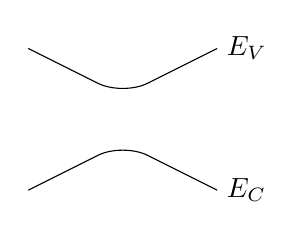
\begin{tikzpicture}[scale = 0.6]
					\begin{scope}[rounded corners = 10pt]
						\draw (0,0) -- (2,1) -- (4,0) node [right] {$E_C$};
						\draw (0,3) -- (2,2) -- (4,3) node [right] {$E_V$};
					\end{scope}
				\end{tikzpicture}
			\end{figure}
		\item
			The following energy diagram describes
			\begin{enumerate}
				\item A semiconductor made entirely of one material.
				\item A semiconductor in which the type of material changes.
				\item A semiconductor in which a voltage is applied across both ends.
				\item Both a and b are correct.
				\item Both a and c are correct.
			\end{enumerate}
			\begin{figure}[H]
				\centering
				\begin{tikzpicture}[scale = 0.6]
					\begin{scope}
						\draw (0,0) -- (4,3) node [right] {$E_C$};
						\draw (0,2) -- (4,5) node [right] {$E_C$};
					\end{scope}
				\end{tikzpicture}
			\end{figure}
	\end{enumerate}
\end{question}

\begin{solution}
	\begin{enumerate}[leftmargin=*]
		\item
			The energy diagram describes \emph{a semiconductor which has variation in doping at the edges and centre}.
		\item
			The energy diagram describes a semiconductor made of a single material, with a voltage applied across it.
			Therefore, \emph{both a and c are correct}.
	\end{enumerate}
\end{solution}

\begin{question}
	A voltage $V$ is applied across a sample of N-type silicon at 300 \kelvin.\\
	The electron drift velocity as a function of electric field is as shown.
	\begin{figure}[H]
		\centering
		\begin{tikzpicture}
			\draw (0,0) rectangle (4,2);
			\draw (-1,1) to [battery1] (0,1);
			\draw (-1,1) -- (-1,0);
			\draw (-1,0) node [ground] {};
			\draw (4,1) -- (5,1);
			\draw (5,1) node [ground] {};
		\end{tikzpicture}
	\end{figure}
	\begin{enumerate}
		\item
			The silicon has the following characteristics.\\
			\begin{align*}
				\text{length } l                 & = 0.1 \si{\centi\metre}                              \\
				\text{cross-sectional area } A   & = 100 \si{\micro\metre\squared}                      \\
				\text{electron mobility } \mu_n  & = 1350 \si{\centi\metre\squared\per\volt\per\second} \\
				\text{dopant concentration } N_D & = 10^{17} \si{\per\centi\metre\cubed}
			\end{align*}
			Calculate the electron drift current $I_{\text{drift}_n}$ with $V = 10 \volt$ applied across the sample.
			Note that the expression for drift current density is
			\begin{align*}
				J_{\text{drift}_n} & = q n \mu_n E
			\end{align*}
			Repeat for a Si sample which is 1 \si{\micro\metre} long.
		\item
			Label the direction of the electric field $\overrightarrow{E}$, and the direction of $J_{\text{drift}_n}$.
		\item
			How much time, on an average, does it take for an electron to drift 1 \si{\micro\metre} in the silicon sample at an electric field of 100 \si{\volt\per\centi\metre}?
			Repeat for $10^5$ \si{\volt\per\centi\metre}.
	\end{enumerate}
\end{question}

\begin{solution}
	\begin{enumerate}[leftmargin=*]
		\item
			If $l = 0.1 \si{\centi\metre}$,
			\begin{align*}
				J_{\text{drift}_n} & = q n \mu_n E                                                                                                                                                                                                               \\
                                                   & = q N_D \mu_n \frac{V}{l}                                                                                                                                                                                                   \\
                                                   & = \left( 1.6 \times 10^{-19} \coulomb \right) \left( 10^{17} \si{\per\centi\metre\cubed} \right) \left( 1350 \si{\centi\metre\squared\per\volt\per\second} \right) \left( \frac{10}{0.1} \si{\volt\per\centi\metre} \right) \\
                                                   & = 2160 \si{\coulomb\per\centi\metre\squared\per\second}                                                                                                                                                                     \\
                                                   & = 2160 \si{\ampere\per\centi\metre\squared}
			\end{align*}
			Therefore,
			\begin{align*}
				I_{\text{drift}_n} & = J_{\text{drift}_n} A                                                                                      \\
                                                   & = \left( 2160 \si{\ampere\per\centi\metre\squared} \right) \left( 100 \si{\micro\metre\squared} \right)     \\
                                                   & = \left( 2160 \si{\ampere\per\centi\metre\squared} \right) \left( 10^{-6} \si{\centi\metre\squared} \right) \\
                                                   & = 2.16 \times 10^{-3} \ampere
			\end{align*}
			If $l = 1 \si{\micro\metre} = 10^{-4} \si{\centi\metre}$,
			\begin{align*}
				J_{\text{drift}_n} & = q n \mu_n E                                                                                                                                                                                                                          \\
                                                   & = q N_D \mu_n \frac{V}{l}                                                                                                                                                                                                              \\
                                                   & = \left( 1.6 \times 10^{-19} \coulomb \right) \left( 10^{17} \si{\per\centi\metre\cubed} \right) \left( 1350 \si{\centi\metre\squared\per\volt\per\second} \right) \left( \frac{10}{0.1} \times10^3 \si{\volt\per\centi\metre} \right) \\
                                                   & = 2160 \times 10^3 \si{\coulomb\per\centi\metre\squared\per\second}                                                                                                                                                                    \\
                                                   & = 2160 \times 10^3 \si{\ampere\per\centi\metre\squared}
			\end{align*}
			Therefore,
			\begin{align*}
				I_{\text{drift}_n} & = J_{\text{drift}_n} A                                                                                                  \\
                                                   & = \left( 2160 \times 10^3 \si{\ampere\per\centi\metre\squared} \right) \left( 100 \si{\micro\metre\squared} \right)     \\
                                                   & = \left( 2160 \times 10^3 \si{\ampere\per\centi\metre\squared} \right) \left( 10^{-6} \si{\centi\metre\squared} \right) \\
                                                   & = 2.16 \ampere
			\end{align*}
		\item
			~\\
			\begin{figure}[H]
				\centering
				\begin{tikzpicture}
					\draw (0,0) rectangle (4,2);
					\draw (-1,1) to [battery1] (0,1);
					\draw (-1,1) -- (-1,0);
					\draw (-1,0) node [ground] {};
					\draw (4,1) -- (5,1);
					\draw (5,1) node [ground] {};

					\draw [-stealth] (1.5,3) -- ++(1,0) node [right] {$\overrightarrow{E}$};
					\draw [-stealth] (1.5,4) -- ++(1,0) node [right] {$\overrightarrow{J_{\text{drift}_n}}$};
				\end{tikzpicture}
			\end{figure}
		\item
			If $E = 10^2 \si{\volt\per\centi\metre}$,
			\begin{align*}
				v_{\text{drfit}_n} & = \mu_n E                                                                                                         \\
                                                   & = \left( 1350 \si{\centi\metre\squared\per\volt\per\second} \right) \left( 100 \si{\volt\per\centi\metre} \right) \\
                                                   & = 1.35 \times 10^5 \si{\centi\metre\per\second}
			\end{align*}
			Therefore, the time required to drift $1 \si{\micro\metre}$ is
			\begin{align*}
				t & = \frac{1 \si{\micro\metre}}{1.35 \times 10^5 \si{\centi\metre\per\second}}       \\
				t & = \frac{10^{-4} \si{\centi\metre}}{1.35 \times 10^5 \si{\centi\metre\per\second}} \\
                                  & = \frac{1}{1.35} \times 10^{-9} \second                                           \\
                                  & = 0.74 \times10^{-9} \second
			\end{align*}
			If $E = 10^5 \si{\volt\per\centi\metre}$,
			\begin{align*}
				v_{\text{drfit}_n} & = \mu_n E                                                                                                                     \\
                                                   & = \left( 1350 \si{\centi\metre\squared\per\volt\per\second} \right) \left( 100 \times 10^3 \si{\volt\per\centi\metre} \right) \\
                                                   & = 1.35 \times 10^8 \si{\centi\metre\per\second}
			\end{align*}
			Therefore, the time required to drift $1 \si{\micro\metre}$ is
			\begin{align*}
				t & = \frac{1 \si{\micro\metre}}{1.35 \times 10^8 \si{\centi\metre\per\second}}       \\
				t & = \frac{10^{-4} \si{\centi\metre}}{1.35 \times 10^8 \si{\centi\metre\per\second}} \\
                                  & = \frac{1}{1.35} \times 10^{-12} \second                                          \\
                                  & = 0.74 \times10^{-12} \second
			\end{align*}
	\end{enumerate}
\end{solution}

\begin{question}
	Consider a particle at $t = 0$ described as a linear combination of two stationary states.
	\begin{align*}
		\Psi(x,0) & = c_1 \psi_1(x) + c_2 \psi_2(x)
	\end{align*}
	where $\psi_1(x)$ and $\psi_2(x)$ are eigenstates of the Hamiltonian, such that
	\begin{align*}
		\hat{H} \psi_1(x) & = E_1 \psi_1(x) \\
		\hat{H} \psi_2(x) & = E_2 \psi_2(x)
	\end{align*}
	In this question assume that the constant $c_1$ and $c_2$ are real.
	\begin{enumerate}
		\item
			What are the physical meaning of ${c_1}^2$ and ${c_2}^2$?
			What can you say about the value of ${c_1}^2 + {c_2}^2$?
		\item
			What is the wave function at subsequent times, i.e. $\Psi(x,t)$?
			Is $\Psi(x,t)$ a stationary state?
			Explain your answer.
		\item
			Find the probability density for the wave function from the previous part.
	\end{enumerate}
\end{question}

\begin{solution}
	\begin{enumerate}[leftmargin=*]
		\item
			${c_1}^2$ represents the probability that the particle has energy $E_1$, and ${c_2}^2$ represents the probability that the particle has energy $E_2$.\\
			As
			\begin{align*}
				\Psi(x,0) & = c_1 \psi_1(x) + c_2 \psi_2(x)
			\end{align*}
			and as the total probability must be $1$,
			\begin{align*}
				{c_1}^2 + {c_2}^2 & = 1
			\end{align*}
		\item
			The eigenvalues of the Hamiltonian are
			\begin{align*}
				E_n & = \frac{n^2 \pi^2 \hbar^2}{2 m a^2}
			\end{align*}
			Therefore,
			\begin{align*}
				E_1 & = \frac{\pi^2 \hbar^2}{2 m a^2} \\
				E_2 & = \frac{4 \pi^2 \hbar^2}{2 m a^2}
			\end{align*}
			Therefore,
			\begin{align*}
				\Psi(x,t) & = \sum\limits_{n} c_n \psi_n(x) e^{-\frac{i E_n t}{\hbar}}                            \\
                                          & = c_1 \psi_1(x) e^{-\frac{i E_1 t}{\hbar}} + c_2 \psi_2(x) e^{-\frac{i E_2 t}{\hbar}} \\
                                          & = c_1 \psi_1(x) e^{-\frac{i \pi^2 \hbar t}{2 m a^2}} + c_2 \psi_2(x) e^{-\frac{4 i \pi^2 \hbar t}{2 m a^2}}
			\end{align*}
			Therefore, as this is not in the form $\psi(x) e^{-\frac{i E t}{\hbar}}$, it is not a stationary state.
		\item
			\begin{align*}
				\left| \Psi(x,t) \right|^2 & = \left| c_1 \psi_1(x) e^{-\frac{i \pi^2 \hbar t}{2 m a^2}} + c_2 \psi_2(x) e^{-\frac{4 i \pi^2 \hbar t}{2 m a^2}} \right|
			\end{align*}
	\end{enumerate}
\end{solution}

\begin{question}
	\begin{enumerate}
		\item
			Consider a classical particle with kinetic energy $E_k$ trapped in an finite square well.
			Neglect friction and any loss of energy due to contact with the wall of the well.
			\begin{enumerate}
				\item Describe the motion of the particle within the well.
				\item Draw the probability of finding the particle as a function of position in the well.
			\end{enumerate}
		\item
			Now consider a quantum particle trapped in an infinite square well.
			Calculate $\langle x \rangle$, $\langle p \rangle$, $\left\langle x^2 \right\rangle$, $\left\langle p^2 \right\rangle$, $\sigma_x$, and $\sigma_p$ for the $n$th stationary state.
		\item
			Using your results from the previous part, verify that the uncertainty principle is satisfied.
	\end{enumerate}
\end{question}

\begin{solution}
	\begin{enumerate}[leftmargin=*]
		\item
			\begin{align*}
				E_k          & = \frac{1}{2} m v^2 \\
				\therefore v & = \sqrt{\frac{2 m}{E_k}}
			\end{align*}
			Therefore, the particle is moving with a velocity $v$.\\
			Therefore, assuming the particle does not collide with any of the walls,
			\begin{align*}
				x & = x_0 + v t
			\end{align*}
			where $x_0$ is the original position of the particle.\\
			Therefore,
			\begin{figure}[H]
				\centering
				\begin{tikzpicture}
					\def\xMIN{0};
					\def\xMAX{5};
					\def\yMIN{0};
					\def\yMAX{3};
					
					\begin{scope}[-stealth]
						\draw (\xMIN,0) -- (\xMAX,0) node [right] {$x$};
						\draw (0,\yMIN) -- (0,\yMAX) node [above] {probability};
					\end{scope}
					
					\begin{scope}
						\draw (\xMIN,\yMAX/2) -- (\xMAX,\yMAX/2);
					\end{scope}
				\end{tikzpicture}
			\end{figure}
		\item
			\begin{align*}
				\psi(x,t) & = \psi(x) e^{-\frac{i E_n t}{\hbar}} \\
                                          & = \sqrt{\frac{2}{a}} \sin\left( \frac{n \pi x}{a} \right) e^{-\frac{i E_n t}{\hbar}}
			\end{align*}
			where
			\begin{align*}
				E_n & = \frac{n^2 \pi^2 \hbar^2}{2 m a^2}
			\end{align*}
			Therefore,
			\begin{align*}
				\psi(x,t) & = \sqrt{\frac{2}{a}} \sin\left( \sqrt{\frac{2 m E_n}{\hbar}} x \right) e^{-\frac{i E_n t}{\hbar}}
			\end{align*}
			Therefore,
			\begin{align*}
				\langle x \rangle & = \int\limits_{-\infty}^{\infty} \psi^*(x,t) x \psi(x,t) \dif t \\
                                                  & = \int\limits_{-\infty}^{\infty} \frac{2}{a} \sin^2 \left( \sqrt{\frac{2 m E_n}{\hbar}} \right) x \dif x
			\end{align*}
			Therefore,
			\begin{align*}
				\left\langle x^2 \right\rangle & = \int\limits_{-\infty}^{\infty} \psi^*(x,t) x^2 \psi(x,t) \dif t \\
                                                               & = \int\limits_{-\infty}^{\infty} \frac{2}{a} \sin^2 \left( \sqrt{\frac{2 m E_n}{\hbar}} \right) x^2 \dif x
			\end{align*}
			Therefore,
			\begin{align*}
				\langle p \rangle & = \int\limits_{-\infty}^{\infty} \psi^*(x,t) \left( -i \hbar \dod{}{x} \psi(x,t) \right) \dif t \\
                                                  & = \int\limits_{-\infty}^{\infty} \sqrt{\frac{2}{a}} \sin\left( \sqrt{\frac{2 m E_n}{\hbar}} x \right) \left( -i \hbar \dod{}{x} \sqrt{\frac{2}{a}} \sin\left( \sqrt{\frac{2 m E_n}{\hbar}} x \right) \right) \dif x
			\end{align*}
			Therefore,
			\begin{align*}
				\left\langle p^2 \right\rangle & = \int\limits_{-\infty}^{\infty} \psi^*(x,t) \left( -i \hbar \dod{}{x} \psi(x,t) \right) \dif t \\
                                                               & = \int\limits_{-\infty}^{\infty} \sqrt{\frac{2}{a}} \sin\left( \sqrt{\frac{2 m E_n}{\hbar}} x \right) \left( -\hbar^2 \dod[2]{}{x} \sqrt{\frac{2}{a}} \sin\left( \sqrt{\frac{2 m E_n}{\hbar}} x \right) \right) \dif x
			\end{align*}
	\end{enumerate}
\end{solution}

\begin{question}
	A particle in an infinite square well is represented, at time $t = 0$ by the following wave function.
	\begin{align*}
		\Psi(x,0) &=
			\begin{cases}
				A x       & ;\quad 0 \le x \le \frac{a}{2} \\
				A (a - x) & ;\quad \frac{a}{2} \le x \le a \\
			\end{cases}
	\end{align*}
	\begin{enumerate}
		\item Find $A$ and sketch $\Psi(x,0)$.
		\item Write an expression for $\Psi(x,t)$.
		\item What is the probability that a measurement of the energy would yield the value $E_1$?
		\item Find $\langle H \rangle$.
	\end{enumerate}
\end{question}

\begin{solution}
	\begin{enumerate}[leftmargin=*]
		\item
			\begin{align*}
				1 & = \int\limits_{-\infty}^{\infty} \left| \Psi(x,0) \right|^2 \dif x                                                                \\
                                  & = \int\limits_{0}^{\frac{a}{2}} A^2 x^2 \dif x + \int\limits_{\frac{a}{2}}^{a} A^2 \left( a^2 - 2 a x + x^2 \right) \dif x        \\
                                  & = \int\limits_{0}^{\frac{a}{2}} A^2 x^2 \dif x + \int\limits_{\frac{a}{2}}^{a} A^2 a^2 - 2 A^2 a x + A^2 x^2 \dif x               \\
                                  & = \left. A^2 \frac{x^3}{3} \right|_{0}^{\frac{a}{2}} + \left. A^2 a^2 x - A^2 a x^2 + A^2 \frac{x^3}{3} \right|_{\frac{a}{2}}^{a} \\
                                  & = A^2 \frac{a^3}{24} + A^2 a^3 - A^2 a^3 + A^2 \frac{a^3}{3} - A^2 \frac{a^3}{2} + A^2 \frac{a^3}{4} - A^2 \frac{a^3}{24}         \\
                                  & = A^2 a^3 \left( \frac{1}{24} + 1 - 1 + \frac{1}{3} - \frac{1}{2} + \frac{1}{4} - \frac{1}{24} \right)                            \\
                                  & = A^2 a^3 \frac{1}{12}
			\end{align*}
			Therefore,
			\begin{align*}
				A^2          & = \frac{12}{a^3} \\
				\therefore A & = \sqrt{\frac{12}{a^3}}
			\end{align*}
			\begin{figure}[H]
				\centering
				\begin{tikzpicture}
					\def\xMIN{0};
					\def\xMAX{5};
					\def\yMIN{0};
					\def\yMAX{3};
					
					\def\A{1};
					\def\a{4};
					
					\begin{scope}[-stealth]
						\draw (\xMIN,0) -- (\xMAX,0) node [right] {$x$};
						\draw (0,\yMIN) -- (0,\yMAX) node [above] {$\Psi(x,0)$};
					\end{scope}
					
					\begin{scope}
						\draw (0,0) -- (\a/2,\A*\a/2) -- (\a,0);
					\end{scope}

					\begin{scope}
						\draw (\a/2,0) circle (1pt) node [below] {$\frac{a}{2}$};
						\draw (0,\A*\a/2) circle (1pt) node [left] {$A \frac{a}{2}$};
					\end{scope}
				\end{tikzpicture}
			\end{figure}
		\item
			\begin{align*}
				\Psi(x,0) & = c_1 \psi_1(x) e^{-\frac{i E_1 t}{\hbar}} + c_2 \psi_2(x) e^{-\frac{i E_2 t}{\hbar}}
			\end{align*}
		\item
			\begin{align*}
				c_n & = \int\limits_{0}^{\frac{a}{2}} \sqrt{\frac{2}{a}} \sin\left( \frac{n \pi x}{a} \right) A x \dif x + \int\limits_{\frac{a}{2}}^{a} A \sqrt{\frac{2}{a}} \sin\left( \frac{n \pi x}{a} \right) (a - x) \dif x
			\end{align*}
			Therefore, solving,
			\begin{align*}
				c_n &=
					\begin{cases}
						0                                                     & ;\quad n \text{ is even} \\
						\sqrt{\frac{2}{a}} \frac{3 A a^2 (-1)^n}{2 n^2 \pi^2} & ;\quad n \text{ is odd}  \\
					\end{cases}
			\end{align*}
			Therefore,
			\begin{align*}
				c_1 & = -\sqrt{\frac{2}{a}} \frac{3 A a^2}{2 \pi^2}
			\end{align*}
			Therefore,
			\begin{align*}
				|c_1|^2 & = \left( -\sqrt{\frac{2}{a}} \frac{3 A a^2}{2 \pi^2} \right)^2 \\
                                        & = \frac{54}{\pi^4}
			\end{align*}
		\item
			\begin{align*}
				\langle H \rangle & = \sum |c_n|^2 E_n \dif x \\
                                                  & = c_1 E_1                 \\
                                                  & = -\sqrt{\frac{2}{a}} \frac{3 A a^2}{2 \pi^2} \frac{\pi^2 \hbar^2}{2 m a^2}
			\end{align*}
	\end{enumerate}
\end{solution}

\end{document}
